\documentclass{article}

\usepackage[final]{neurips_2024}
\makeatletter
\renewcommand{\@notice}{}
\makeatother

\usepackage[utf8]{inputenc} % allow utf-8 input
\usepackage[T1]{fontenc}    % use 8-bit T1 fonts
\usepackage{hyperref}       % hyperlinks
\usepackage{url}            % simple URL typesetting
\usepackage{booktabs}       % professional-quality tables
\usepackage{amsfonts}       % blackboard math symbols
\usepackage{amsmath}        % math environments
\usepackage{nicefrac}       % compact symbols for 1/2, etc.
\usepackage{microtype}      % microtypography
\usepackage{xcolor}         % colors
\usepackage{graphicx}       % figures

\usepackage{bm}

\usepackage[inline]{enumitem}

% \setcounter{secnumdepth}{0}

\title{Introducing Shepherd, a reinforcement learning based rocket hovering model
\thanks{Code available at \url{https://github.com/andrei-vilcan/shepherd-hover}.}}


\author{%
  Andrei O. Vilcan \\
  Radboud Universiteit \\
  Houtlaan 4, Nijmegen, 6525XZ
 \\
  \texttt{andrei.vilcan@ru.nl} \\
}


\begin{document}

\maketitle

\begin{abstract}

We present Shepherd, a model-free actor-critic agent that learns to stabilize a rocket against the force of gravity in a simulated two-dimensional physics environment. The method we use to train the agent is the episodic REINFORCE algorithm, augmented with Generalized Advantage Estimation (GAE) and extended with curriculum learning, training on subsets of the final task with increasing difficulty. Our key finding is that for this task, GAE, which reduces the effective lookahead, is essential for stable training. 

\end{abstract}


\section{Introduction}

Stabilizing a rocket in a constant hover at a particular location in space is a demanding continuous control problem - one that involves fine and rapid adjustments taking into consideration the effect of one's actions on position, velocity, angle, and angular velocity, in order to both counteract the force of gravity and keep the rocket in a stable position.
In this work, the research question we address is as follows: Can a model-free policy-gradient actor-critic reinforcement-learning agent stabilize a rocket in a two-dimensional simulated gravitational environment?
We further augment the REINFORCE algorithm~\citep{williams1992} with Generalized Advantage Estimation (GAE)~\citep{schulman2016} and train the agent with a difficulty-scaled curriculum, overall improving the agent's performance and arriving at a more robust policy.


\section{Methods}

% \subsection{Preliminaries}
\subsection{Environment}

% \paragraph{Environment}

First, we implement a two-dimensional rocket hovering Gymnax environment.

\paragraph{State}

The state of the system is fully described by 12 variables, one of which is time; the timestep is $0.02$ seconds, and there is a maximum episode length of $1000$ timesteps, or $20$ seconds. The rocket's position and orientation are described by cartesian coordinates $(x, y)$ and an angle $\theta$ respectively; its linear and angular velocity are described by $(\dot x, \dot y)$ and $\omega$ respectively.
The rocket has one main thruster placed on the bottom, which faces downwards, and thrust is described by a scalar $\tau$. The thruster's gimbal (orientation relative to the rocket) is further described by an angle g. In addition, the rocket has two small thrusters near the top, one on either side, for balancing. The fuel remaining in the rocket is described by a variable f.

\paragraph{Actions}

The agent outputs 4 dimensional continuous actions in the range of [-1, 1], with each dimension corresponding to one of the following: the throttle of the main booster, the gimbal angle of the main booster, and the throttle of the left and right boosters. These are then mapped to the range [0, 1], in the case of the booster throttles, and to the range of [-0.3 rad, 0.3 rad] in the case of the gimbal.

\paragraph{Physics}

Throughout the whole environment, there is a constant downwards gravitational force exerted on the rocket equal to that present on Earth, of $9.81\,\text{m/s}^2$.
The rocket has a height $h = 10\,\text{m}$, a mass $m = 1000\,\text{kg}$, and a moment of inertia $I = 10{,}000\,\text{kg}\!\cdot\!\text{m}^2$. The main thruster has a maximum thrust of $20{,}000\,\text{N}$, whereas the side thrusters have a maximum thrust of $500\,\text{N}$, and they are placed $5$ meters up from the center of the rocket, on each side. All thrusters influence the positional and rotational velocity of the rocket according to the equations below.

\begin{equation}
    \ddot{x} = \frac{F_\text{main} \sin(\theta + g) + F_\text{side} \cos\theta}{m}, \qquad
    \ddot{y} = -g_\text{grav} + \frac{F_\text{main} \cos(\theta + g) + F_\text{side} \sin\theta}{m}
    \label{eq:dynamics_xy}
\end{equation}
\begin{equation}
    \ddot{\theta} = \frac{F_\text{main} \sin(g) \cdot d_m + F_\text{side} \cdot d_s}{I}
    \label{eq:dynamics_theta}
\end{equation}

where $F_\text{side} = F_\ell - F_r$ is the net lateral force from the auxiliary thrusters, and $d_m$, $d_s$ are the distances of the main engine and side thrusters from the center of mass.

\paragraph{Observation}

The agent observes an $11$-dimensional vector as its input, which contains the state variables. The agent has perfect observability over these variables, and the positions, velocities, orientation, angular velocity, gimbal, and fuel are each normalized by constants $c_x, c_y, c_v, c_{\omega}$, with each constant calculated according to a respective formula as a function of an offset factor defined in the curriculum.

\begin{equation}
    \mathbf{o} = \left[\frac{x}{c_x},\; \frac{y}{c_y},\; \frac{\dot{x}}{c_v},\; \frac{\dot{y}}{c_v},\; \frac{\theta}{\pi},\; \frac{\omega}{c_\omega},\; \tau,\; \frac{g}{g_\text{max}},\; \ell,\; r,\; \frac{f}{f_{max}}\right]
\end{equation}

\paragraph{Reward}

The reward the agent receives at each time step as a function of the state variables is calculated as the weighted sum of the exponential of the negative difference between the target value and the present value for the position, velocity, angle, and angular velocity. Generally, this means that being close to the origin (the target), having low velocity, being upright, and having a low angular velocity are rewarded in an exponentially decaying manner. Specifically, the reward is calculated according to the following equation,

\begin{equation}
    r_t = \alpha_d \exp\!\left(\frac{-d_t}{5}\right) + \alpha_v \exp\!\left(\frac{-v_t}{5}\right) + \alpha_\theta \exp\!\left(\frac{-|\theta_t|}{0.5}\right) + \alpha_\omega \exp\!\left(\frac{-|\omega_t|}{1}\right)
\end{equation}

where $d_t = \sqrt{x_t^2 + y_t^2}$ is the distance, $v_t = \sqrt{\dot{x}_t^2 + \dot{y}_t^2}$ is the velocity, and the reward factors $(\alpha_d, \alpha_v, \alpha_\theta, \alpha_\omega) = (2, 1, 1, 1)$ specify the importance of each measure in the calculation. The per-component reward curves are shown in Figure~\ref{fig:reward_structure} in the Appendix.


\subsection{REINFORCE Algorithm}

\paragraph{Policy Network (Actor)}

The policy $\pi$ generates actions by sampling from Gaussian distributions, whose means $\bm{\mu} \in \mathbb{R}^4$ are calculated as a function of the observation $\mathbf{o}$, through a multi-layer perceptron (MLP) with hidden layers of sizes $256, 128$, using the $\tanh$ activation function between layers, as well as a final $\tanh$, bounding outputs to $[-1, 1]$. Meanwhile, the logarithm of the standard deviations $\log \bm{\sigma}$ are learnable parameters as well and control the amount of exploration the agent can perform. Actions are sampled by calculating the value of the following variable.

\begin{equation}
  \mathbf{a}_t = \text{clip}(\tilde{\mathbf{a}}_t,\; -1,\; 1), \qquad \tilde{\mathbf{a}}_t \sim \mathcal{N}\!\big(\bm{\mu}_\phi(\mathbf{o}_t),\; \text{diag}(\bm{\sigma}^2)\big)
  \label{eq:action_dist}
\end{equation}

where $\bm{\mu}_\phi(\mathbf{o}_t)$ is the MLP output, and $\bm{\sigma} = \exp(\log \bm{\sigma})$ with $\log \bm{\sigma}$ clipped to $[-2.0, 0.5]$.

\paragraph{Value Network (Critic)}

A separate network outputs a single scalar, calculating an estimate for the value of being in a certain state via a MLP with hidden layers of sizes $256, 128$, using $\tanh$ activation functions between layers.

\paragraph{Generalized Advantage Estimation}

We estimate the advantage function using the methodology described in \citet{schulman2016}. First, we obtain the TD residual of $V$ with discount $\gamma$ as $\delta_t = r_t + \gamma V(\mathbf{o}_{t+1}) - V(\mathbf{o}_t)$, where $V$ is the estimated value of the state $\mathbf{o}_t$. Then, we calculate the GAE according to the following formula~\citep[Eq.~16]{schulman2016}:

\begin{equation}
    \hat{A}_t^{\text{GAE}(\gamma, \lambda)} = \sum_{l=0}^{\infty} (\gamma \lambda)^l \, \delta_{t+l}
    \label{eq:gae}
\end{equation}

Note, setting $\lambda = 1$, we obtain the episodic REINFORCE policy gradient algorithm with the value function as a baseline ~\citep{williams1992}. Comparatively, using $\lambda < 1$ we introduce a small amount of bias with the benefit of reduced variance of the advantage~\citep{schulman2016}.

\paragraph{Value Estimation}


After this, we must recover the returns; to obtain an estimate, we perform, as per the suggestion in ~\citep{schulman2016}:

\begin{equation}
    \hat{G}_t = \hat{A}_t + V_\psi(\mathbf{o}_t)
    \label{eq:lambda_return}
\end{equation}

\paragraph{Policy Gradient}

The actor is trained by minimizing the REINFORCE policy loss~\citep{williams1992}: the product of the mean negative log-likelihood and the estimated advantage.

\begin{equation}
  \mathcal{L}_\pi(\phi) = -\frac{1}{N} \sum_{i=1}^{N}
  \frac{1}{|\mathcal{T}_i|}\sum_{t \in \mathcal{T}_i}
  \log \pi_\phi(\mathbf{a}_t^{(i)} \mid \mathbf{o}_t^{(i)}) \, \hat{A}_t^{(i)}
  \label{eq:policy_loss}
\end{equation}

Meanwhile, the critic is trained by minimizing the value loss function: the mean-square-error between predicted values and estimated returns.

\begin{equation}
  \mathcal{L}_V(\psi) = \frac{1}{\sum_i |\mathcal{T}_i|}
  \sum_{i=1}^{N} \sum_{t \in \mathcal{T}_i}
  \left(V_\psi(\mathbf{o}_t^{(i)}) - \hat{G}_t^{(i)}\right)^2
  \label{eq:value_loss}
\end{equation}

\subsection{Curriculum Learning}

\paragraph{Curriculum Stages}

To bring to a hover at a specific target a rocket that is dealing with arbitrary fluctuations in its position, velocity, orientation, and angular velocity, is certainly a more difficult task than to teach one that is already in the target state. In the first stage of the curriculum, we train the rocket to hover, starting in an upright position at the origin, and with zero (angular) velocity. In the second stage, using a scaling factor, we slowly increase the difficulty of the task until the maximum perturbations are as follows: maximum distance is $20\,\text{m}$, velocity $10\,\text{m/s}$, orientation $0.3$ radians, and angular velocity $0.5$ radians. In the third and final stage of the curriculum, the state variables are initialized according to maximum perturbation values. Each curriculum phase has $100{,}000$ episodes.

\paragraph{Difficulty Coefficient}

Using a progressively increasing difficulty coefficient during the second stage, we smoothly transition between the first and last stages. We scale the difficulty of the task by multiplying the maximum initial perturbation values by the output of the function $c(p) = \frac{1}{1 + \exp(-e^e \cdot (p - \nicefrac{1}{2}))}$, where $p$ is the normalized progress in this stage of the curriculum. This function is visualized in Figure~\ref{fig:difficulty} in the Appendix.


\section{Results}

We train the agent for $300{,}000$ episodes in batches of 16, resulting in the training curves in Figure~\ref{fig:training_curves}.

\begin{figure}[h]
  \centering
  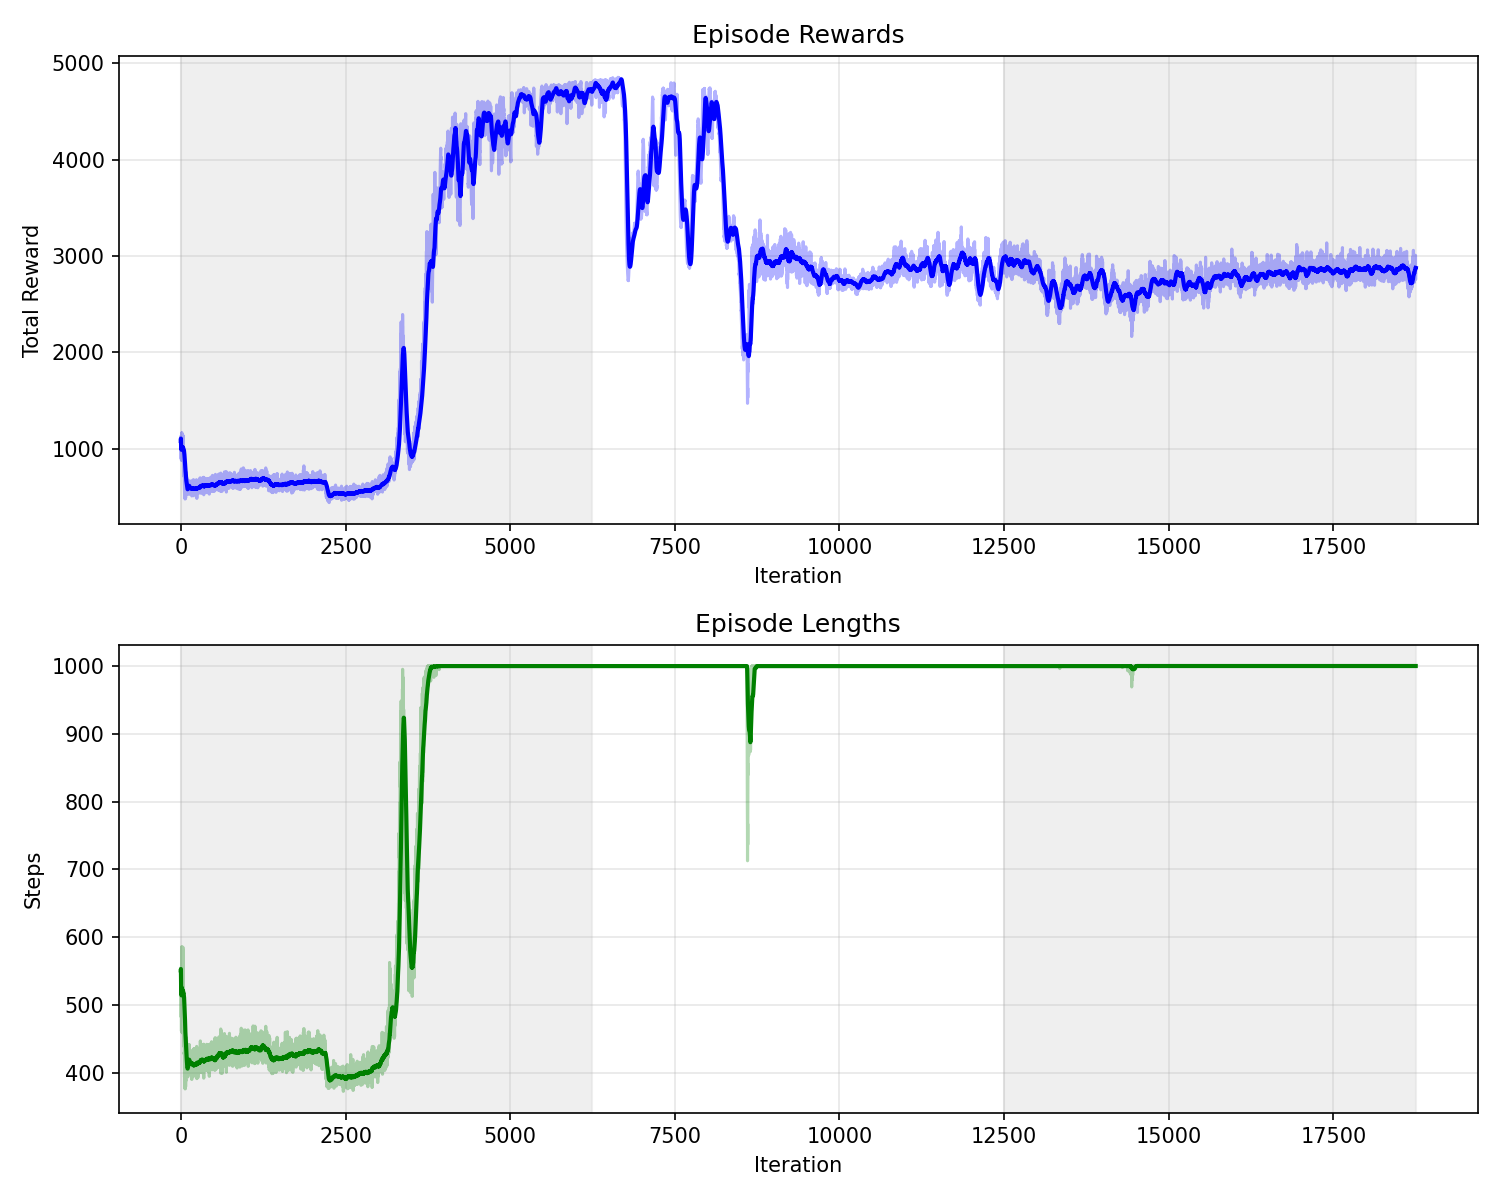
\includegraphics[width=0.9\linewidth]{training_curves.png}
  \caption{Training curves over $300{,}000$ episodes in batches of 16. Shading alternates between and indicates curriculum stages.}
  \label{fig:training_curves}
\end{figure}

\subsection{Training Stages}

In the first stage, we initially observe the rocket falling due to gravity and leaving the bounds, ending the episode. At around $3{,}750$ iterations, we can see the agent beginning to control the rocket, and the average episodic reward rises to near $5{,}000$.
In the early episodes of stage two, with the introduction of light perturbations, we observe a dip in the average reward.
Starting in stage three, under full perturbation the agent stabilizes, and the average reward stays moderately consistent throughout the stage.


\subsection{Final Performance}

By the end of training, the agent achieves an average episodic reward of $2{,}774.3$ throughout the third stage, which is higher than $2{,}173.6$ the average episodic reward of the first stage. However, during the third stage the agent is still not able to achieve as high of an average reward as in the second half of the first stage, since perturbations limit the maximum potential reward. Interestingly, the second stage has the highest average reward of $3{,}263.0$.

\section{Discussion}

\subsection{Generalized Advantage Estimation}

Using GAE with $\lambda = 0.95$, the agent was able to stabilize during all stages. Comparatively, with $\lambda = 1$, the average rewards are much lower, and qualitatively speaking, the agent was unable to stabilize the rocket in any of the stages.

\subsection{Curriculum Learning}

The curriculum used in this experiment is only viable as the tasks of the earlier stages are a subset of the tasks in the later stages, i.e.\ hovering a rocket at a point is a subset of bringing the rocket to that point and then hovering it.

\subsection{Reward Design}

The critical feature of this reward function that allowed the agent to effectively use it to represent the value of a point in the state space is it being differentiable everywhere.

\subsection{Future Work}

Natural extensions of this project include the following: (1) creating a rocket landing environment with a target and extending the curriculum to include this training; (2) increasing the maximum perturbation and height values for the hovering and landing environments respectively; (3) more closely simulating a real physical environment, for example by adding air resistance, wind noise, a minimum throttle value, and reducing to partial observability; (4) further extending the landing environment to include orbital mechanics and training the agent to land from orbit around a celestial mass.


\begin{thebibliography}{99}

\bibitem[Schulman et~al.(2016)Schulman, Moritz, Levine, Jordan, and Abbeel]{schulman2016}
J.~Schulman, P.~Moritz, S.~Levine, M.~Jordan, and P.~Abbeel.
\newblock High-dimensional continuous control using generalized advantage estimation.
\newblock In \emph{International Conference on Learning Representations (ICLR)}, 2016.

\bibitem[Williams(1992)]{williams1992}
R.~J. Williams.
\newblock Simple statistical gradient-following algorithms for connectionist reinforcement learning.
\newblock \emph{Machine Learning}, 8(3):229--256, 1992.

\end{thebibliography}

\newpage
\appendix
\section{Appendix}

\subsection{Reward Structure}

\begin{figure}[h]
  \centering
  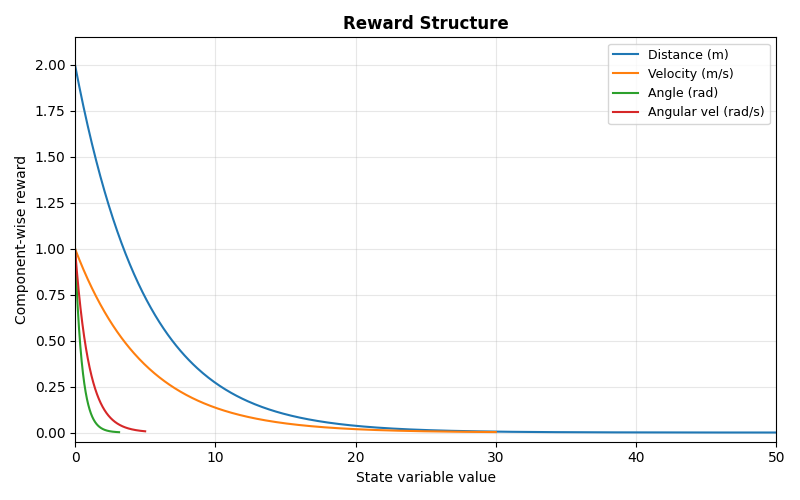
\includegraphics[width=0.85\linewidth]{reward_structure.png}
  % \caption{Per-component reward values as a function $r(c) = \alpha_i \cdot \exp(-x_i / \tau_i)$ of the respective state variable.}
  \caption{Reward as a function of respective state variable.}
  \label{fig:reward_structure}
\end{figure}

\subsection{Difficulty Coefficient}

\begin{figure}[h]
  \centering
  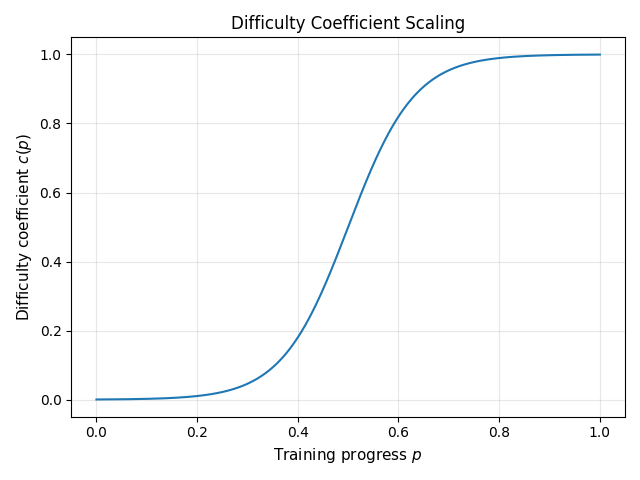
\includegraphics[width=0.7\linewidth]{difficulty_coefficient.png}
  \caption{Sigmoid difficulty schedule $c(p) = \frac{1}{1 + e^{-e^e(p - 1/2)}}$ used in Stage 2 of the curriculum.}
  \label{fig:difficulty}
\end{figure}

\newpage
\subsection{Hyperparameter Summary}

\begin{table}[h]
\centering
\begin{tabular}{@{}ll@{}}
\toprule
Hyperparameter & Value \\
\midrule
Discount factor $\gamma$ & 0.99 \\
GAE $\lambda$ & 0.95 \\
Policy learning rate & $3 \times 10^{-4}$ \\
Value learning rate & $1 \times 10^{-3}$ \\
Optimizer & Adam \\
Batch size (parallel episodes) & 16 \\
Policy hidden layers & {[256, 128]} \\
Value hidden layers & {[256, 128]} \\
Activation function & $\tanh$ \\
Max steps per episode & 1{,}000 \\
Time step $\Delta t$ & 0.02\,s \\
Curriculum stages & $3 \times 100{,}000$ episodes \\
\bottomrule
\end{tabular}
\caption{Hyperparameters used for training.}
\label{tab:hyperparams}
\end{table}


\end{document}
